%\usetikzlibrary{arrows.meta,shapes,positioning,shadows,trees,decorations.pathmorphing}

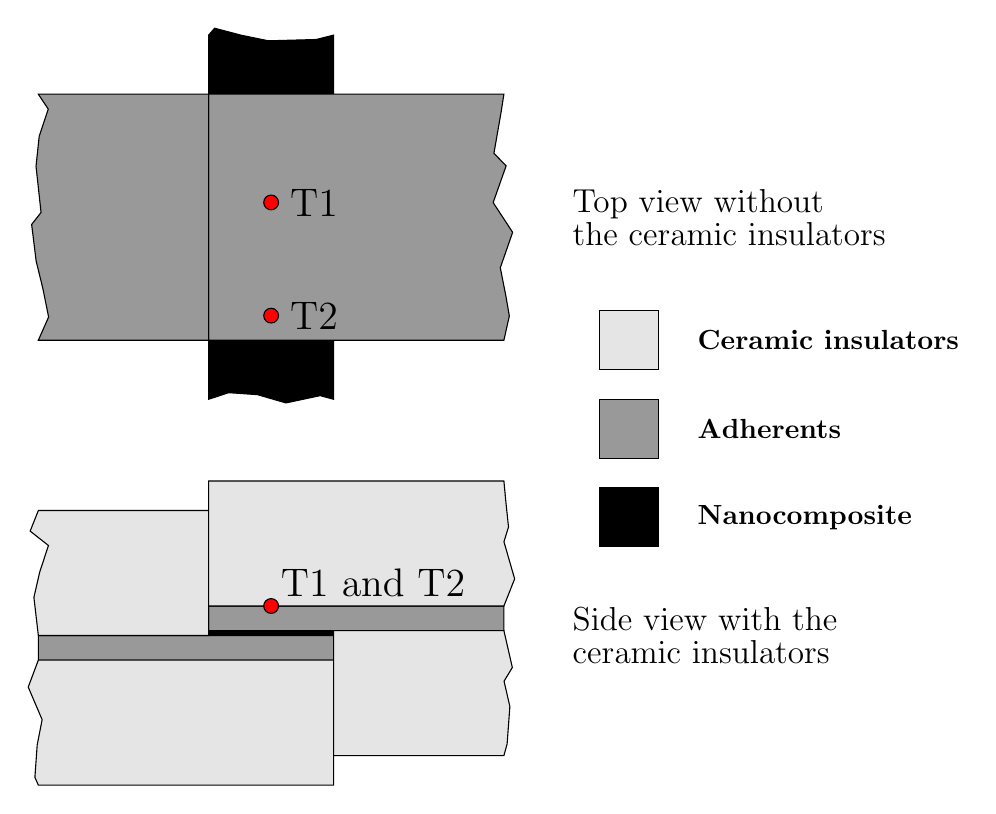
\begin{tikzpicture}[scale=0.125]

%Couleurs
\def \colceramique{black!10}
\def \colcomposite{black!40}

\def \legend{6}

%Définition des dimensions du joint soudé
\def \overlap{12.7}
\def \epceramique{12.7}
\def \epcomposite{2.5}
\def \epnanocomposite{0.5}
\def \longueur{30}
\def \gapfigure{30}
\def \largeursoudure{25}
\def \depassementsoudure{6}
\def \diacercle{0.75}

%%%Vue du dessus %%%
\draw (\longueur+\depassementsoudure,\gapfigure+0.5*\largeursoudure) node [right, align=left]{\large Top view without \\ \large the ceramic insulators};

%Élément chauffant
\draw[black,decoration={random steps, amplitude=4, segment length=10},fill=black] (0,\gapfigure-\depassementsoudure) decorate{-- ++(\overlap,0)} -- ++(0,2*\depassementsoudure+\largeursoudure) decorate{-- ++(-\overlap,0)} -- cycle;

%Adhérent
\draw[black,decoration={random steps, amplitude=4, segment length=10},fill=\colcomposite] 
(0,\gapfigure) -- ++(\longueur,0) decorate{-- ++(0,\largeursoudure)} -- ++(-\longueur,0) -- cycle;
\draw[black,decoration={random steps, amplitude=4, segment length=10},fill=\colcomposite] 
(0,\gapfigure) -- ++(-\longueur+\overlap,0) decorate{-- ++(0,\largeursoudure)} -- ++(\longueur-\overlap,0) -- cycle;

%Position du thermocouple
\draw[fill=red] (0.5*\overlap,\gapfigure+14) circle (0.75) node [right]{\ \Large T1};
\draw[fill=red] (0.5*\overlap,\gapfigure+2.5) circle (0.75) node [right]{\ \Large T2};


%%% Vue du côté %%%
\draw (\longueur+\depassementsoudure,0) node [right, align=left]{\large Side view with the \\ \large ceramic insulators};

%Éléments chauffants
\draw[black,thick,fill=black] (0,0) -- ++(\overlap,0) -- ++(0,\epnanocomposite) -- ++(-\overlap,0) -- cycle;

%Adhérents
\draw[black,decoration={random steps, amplitude=4, segment length=6},fill=\colcomposite] 
(\overlap,0) -- ++(-\longueur,0) decorate{-- ++(0,-\epcomposite)} -- ++(\longueur,0) -- cycle;
\draw[black,decoration={random steps, amplitude=4, segment length=6},fill=\colcomposite] 
(0,\epnanocomposite) -- ++(\longueur,0) decorate{-- ++(0,\epcomposite)} -- ++(-\longueur,0) -- cycle;

%Céramiques
\draw[black,decoration={random steps, amplitude=4, segment length=10},fill=\colceramique] 
(\overlap,-\epcomposite) -- ++(-\longueur,0) decorate{-- ++(0,-\epceramique)} -- ++(\longueur,0) -- cycle;
\draw[black,decoration={random steps, amplitude=4, segment length=10},fill=\colceramique] 
(0,0) -- ++(-\longueur+\overlap,0) decorate{-- ++(0,\epceramique)} -- ++(\longueur-\overlap,0) -- cycle;
\draw[black,decoration={random steps, amplitude=4, segment length=10},fill=\colceramique] 
(\overlap,\epnanocomposite) -- ++(\longueur-\overlap,0) decorate{-- ++(0,-\epceramique)} -- ++(-\longueur+\overlap,0) -- cycle;
\draw[black,decoration={random steps, amplitude=4, segment length=10},fill=\colceramique] 
(0,\epnanocomposite+\epcomposite) -- ++(\longueur,0) decorate{-- ++(0,\epceramique)} -- ++(-\longueur,0) -- cycle;

%Position du thermocouple
\draw[fill=red] (0.5*\overlap,\epnanocomposite+\epcomposite) circle (0.75) node [above right]{\Large T1 and T2};

%Legend
\begin{scope}[shift={(\overlap+\longueur-0.5*\legend,\gapfigure+0.5*\legend)}]
	\begin{scope}[shift={(0,0)}]
		\draw [black, fill=\colceramique] (0,0) rectangle ++(\legend,-\legend);
		\draw (1.5*\legend,-0.5*\legend) node[right]{{\textbf{Ceramic insulators}}} ;
	\end{scope}

	\begin{scope}[shift={(0,-1.5*\legend)}]
		\draw [black, fill=\colcomposite] (0,0) rectangle ++(\legend,-\legend);
		\draw (1.5*\legend,-0.5*\legend) node[right]{{\textbf{Adherents}}} ;
	\end{scope}

	\begin{scope}[shift={(0,-3*\legend)}]
		\draw [black, fill=black] (0,0) rectangle ++(\legend,-\legend);
		\draw (1.5*\legend,-0.5*\legend) node[right]{{\textbf{Nanocomposite}}} ;
	\end{scope}
\end{scope}

\end{tikzpicture}
